%%%%%%%%%%%%%%%%%%%%%%%%%%%%%%%%%%%%%%%%%%%%%%%%%%%%%%%%%%%%%%%%%%%%%%%%%%%%%%%%%%%%
% Document data
%%%%%%%%%%%%%%%%%%%%%%%%%%%%%%%%%%%%%%%%%%%%%%%%%%%%%%%%%%%%%%%%%%%%%%%%%%%%%%%%%%%%
\documentclass[12pt]{article} %report allows for chapters
%%%%%%%%%%%%%%%%%%%%%%%%%%%%%%%%%%%%%%%%%%%%%%%%%%%%%%%%%%%%%%%%%%%%%%%%%%%%%%%%%%%%
\usepackage{preamble}
\newcommand{\grad}{\boldsymbol{\vec{\nabla}}}
\newcommand{\vecfieldB}{\boldsymbol{\vec{B}}}
\newcommand{\vecfieldE}{\boldsymbol{\vec{E}}}
\newcommand{\rhat}{\boldsymbol{\hat{r}}}
\newcommand{\thetahat}{\boldsymbol{\hat{\theta}}}
\newcommand{\phihat}{\boldsymbol{\hat{\phi}}}
\newcommand{\rhohat}{\boldsymbol{\hat{\rho}}}

\begin{document}

\begin{center}
   \textsc{\large MATH 272, Homework 4. \emph{Solutions}.}\\
\end{center}
\vspace{.5cm}

\begin{problem}
    Plot each of the following vector fields. Describe what each field represents in the relevant coordinate system. Do we see any points in space where there are issues with these vector fields?
    \begin{enumerate}[(a)]
        \item $\rhohat = \frac{x}{\sqrt{x^2+y^2}}\xhat + \frac{y}{\sqrt{x^2+y^2}}\yhat$.
        \item $\thetahat = \frac{-y}{\sqrt{x^2+y^2}}\xhat + \frac{x}{\sqrt{x^2+y^2}}\yhat$.
        \item $\phihat = \frac{xz}{\sqrt{x^2+y^2}\sqrt{x^2+y^2+z^2}}\xhat + \frac{yz}{\sqrt{x^2+y^2}\sqrt{x^2+y^2+z^2}}\yhat-\frac{\sqrt{x^2+y^2}}{\sqrt{x^2+y^2+z^2}}\zhat$.
        \item $\rhat = \frac{x}{\sqrt{x^2+y^2+z^2}}\xhat + \frac{y}{\sqrt{x^2+y^2+z^2}}\yhat+\frac{z}{\sqrt{x^2+y^2+z^2}}\zhat$.
    \end{enumerate}
\end{problem}
\begin{solution}~
\begin{enumerate}[(a)]
    \item Here is a plot of $\rhohat$.
    \begin{figure}[H]
        \centering
        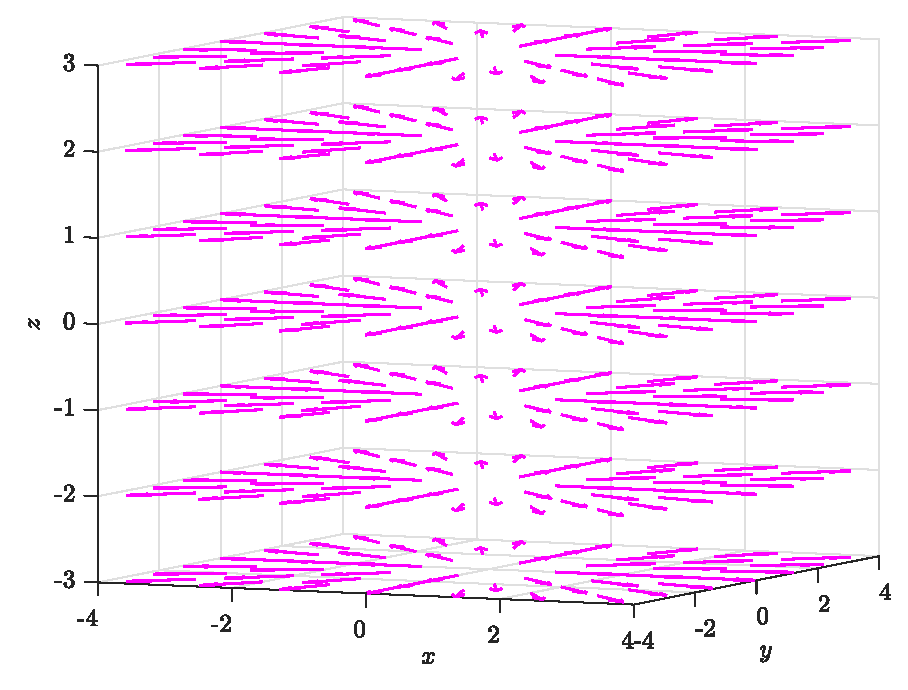
\includegraphics[width=.6\textwidth]{figures/rho_hat}
    \end{figure}
    Notice that when $x=y=0$ (i.e., along the $z$-axis) that we have an inability to ascribe a direction to $\rhohat$. This is because the coordinate $\rho$ itself is defined to be the measurement of distance from the $z$-axis. The field $\rhohat$ points in the direction in which $\rho$ increases most quickly (i.e., it points along $\grad \rho(x,y,z)$). Since any direction satisfies this idea, there is no unique direction to choose. This vector field is unable to describe anything useful along the $z$-axis.

    \item Here is a plot of $\thetahat$.
    \begin{figure}[H]
        \centering
        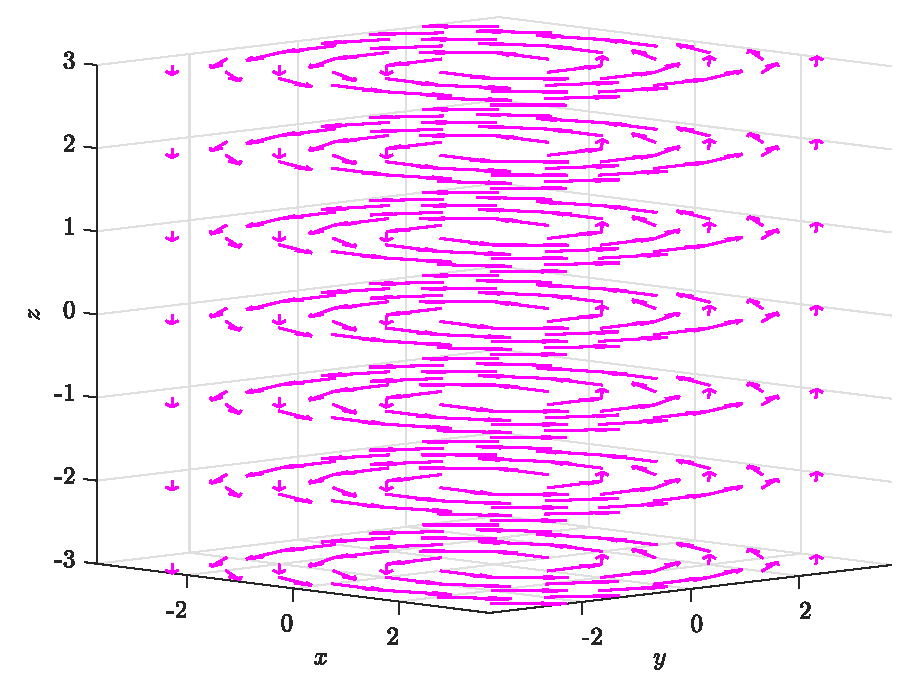
\includegraphics[width=.6\textwidth]{figures/theta_hat}
    \end{figure}
    Much like $\rhohat$, $\thetahat$ has issues along the $z$-axis. But, the reason for issue is subtly different than the failure of $\rhohat$. If we pick a point with $x\neq 0$ or $y\neq 0$, then we can ascribe an angle to this vector relative to the $xz$-plane. However, for points on the $z$-axis, there is no angle to speak of -- it isn't that it is a zero angle, it simply does not exist. 

    \item Here is a plot of $\phihat$.
    \begin{figure}[H]
        \centering
        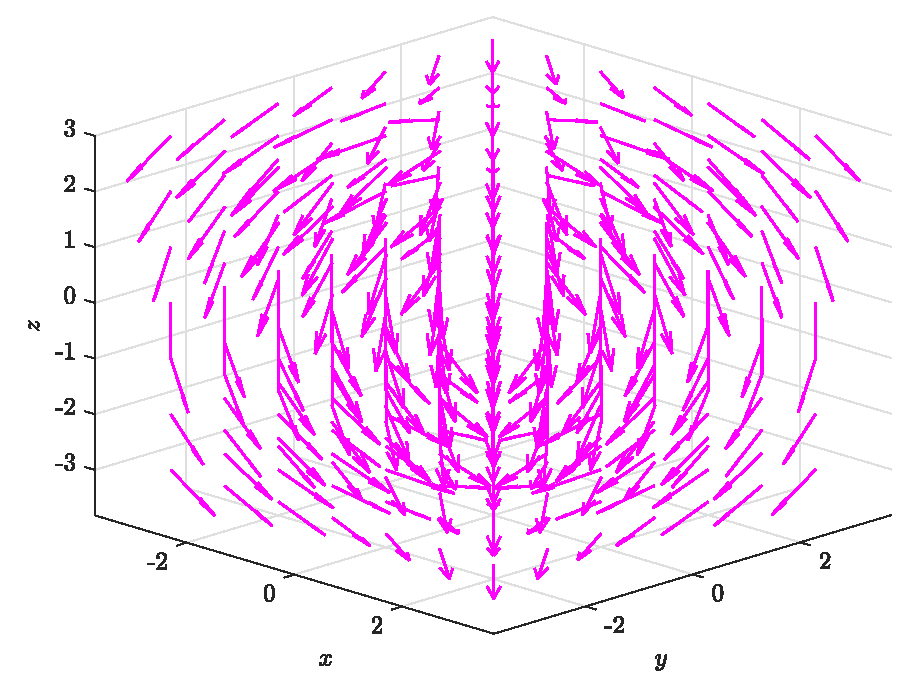
\includegraphics[width=.6\textwidth]{figures/phi_hat}
    \end{figure}
    This vector field again lacks a description along the $z$-axis since we would have $x=y=0$. Once again, the reasoning here is subtle yet important. A point on the $z$-axis either has an angle of $\phi = 0$ or $\phi = \pi$ and, for the origin, there isn't a valid angle to specify there either. Once again, we can think about what direction moving away from the $z$-axis would increase $\phi$ (i.e., point in $\phihat$), and the answer is \emph{every} direction does this. 

    \item Here is a plot of $\rhat$.
    \begin{figure}[H]
        \centering
        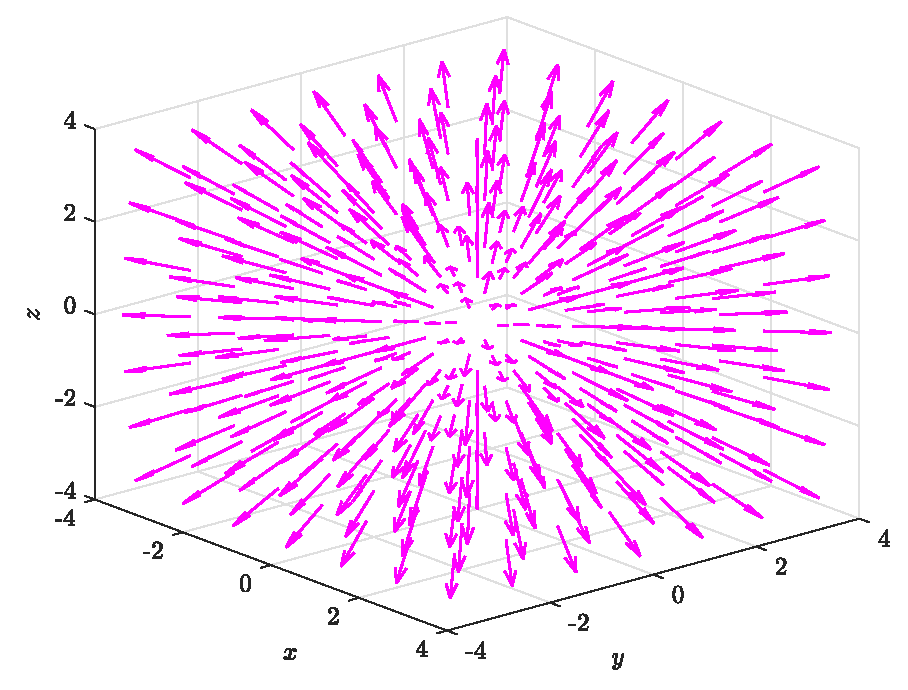
\includegraphics[width=.6\textwidth]{figures/r_hat}
    \end{figure}
    This field experiences only a single point of concern. Namely, the origin. There, this field is not defined as any direction we choose to move at the origin increases $r$ since $r$ is a measure of distance from the origin. 
\end{enumerate}
\end{solution}

\newpage
\begin{problem}
Let us see some of the usefulness of cylindrical coordinates.
\begin{enumerate}[(a)]
    \item Using the fact that $\thetahat = \frac{-y}{\sqrt{x^2+y^2}}\xhat + \frac{x}{\sqrt{x^2+y^2}}\yhat$, convert the magnetic field 
    \[
    \vecfieldB = -\frac{y}{2}\xhat + \frac{x}{2}\yhat,
    \]
    into cylindrical coordinates (i.e., only a function of $\rho$, $\theta$, $z$, and $\rhohat$, $\thetahat$, and $\zhat$).  
        \item Parameterize a curve $\curvegamma(t)$ that traces out the unit circle in the $xy$-plane in cylindrical coordinates.
        \item Compute the tangent vector $\tangentgamma(t)$ in cylindrical coordinates?
        \item Compute the following integral using cylindrical coordinates
        \[
        \int_{\curvegamma} \vecfieldB \cdot d\curvegamma.
        \]
\end{enumerate}
\end{problem}
\begin{solution}~
\begin{enumerate}[(a)]
    \item We have that
    \[
    \vecfieldB = -\frac{y}{2} \xhat + \frac{x}{2}\yhat.
    \]
    Then, note that we have
    \begin{align*}
        \vecfieldB &= \frac{1}{2}\sqrt{x^2+y^2} \left( \frac{-y}{\sqrt{x^2+y^2}} \xhat + \frac{x}{\sqrt{x^2+y^2}} \right)\\
        &=\frac{1}{2} \sqrt{x^2+y^2} \thetahat.
    \end{align*}
    Finally, we have that $\rho = \sqrt{x^2+y^2}$ and hence
    \[
    \vecfieldB = \frac{\rho}{2} \thetahat.
    \]
    \item It suffices to find functions $\rho(t)$, $\theta(t)$, and $z(t)$ to create the curve
    \[
    \curvegamma(t) = \rho(t) \rhohat + \theta(t) \thetahat + z(t) \zhat.
    \]
    Note that for a circle centered along the $z$-axis, we have that $\rho$ is constant and in this case since we are considering the unit circle, we have $\rho(t)=1$.  Similarly, we want the circle to lie in the $xy$-plane where $z=0$, hence we must have $z(t)=0$.  Finally, we must trace the whole unit circle so we must have $\theta$ cover all of $[0,2\pi)$. One choice is to have $\theta(t)=t$ for $t\in[0,2\pi)$, but there are many other options! Using these choices, we have
    \[
    \curvegamma(t) = \rhohat + t \thetahat.
    \]
    \item Then, we have the tangent vector $\tangentgamma = \frac{d\curvegamma}{dt}$ and thus
    \[
    \tangentgamma(t) = \thetahat.
    \]
    \item Note that from the above work we have
    \[
    d \curvegamma = \tangentgamma dt = \thetahat dt.
    \]
    Thus, 
    \[
    \vecfieldB \cdot \tangentgamma = \frac{\rho}{2}.
    \]
    This gives us that
    \begin{align*}
        \int_{\curvegamma} \vecfieldB \cdot d\curvegamma &= \int_0^{2\pi} \frac{\rho(t)}{2}dt\\
        &=\int_0^{2\pi} \frac{1}{2} dt\\
        &= \pi.
    \end{align*}
    Above, we can note that $\rho(t)=1$ since we are integrating along the unit circle in the $xy$-plane.
\end{enumerate}
\end{solution}

\newpage
\begin{problem}
    Convert the following integrals to integrals in cylindrical coordinates. Also, describe the region in which you are integrating over. Do not evaluate the integrals.
    \begin{enumerate}[(a)]
        \item $\displaystyle{\int_{-1}^{1} \int_{-1}^{1} \int_{-\sqrt{1-y^2}}^{\sqrt{1-y^2}} xyz dxdydz}$.
        \item $\displaystyle{\int_0^1 \int_{-z}^z \int_{-\sqrt{z^2-y^2}}^{\sqrt{z^2-y^2}} x^2+y^2+z^2 dxdydz}$.
    \end{enumerate}
\end{problem}
\begin{solution}~
\begin{enumerate}[(a)]
    \item First, let us convert the integrand to cylindrical coordinates. We have
    \[
    xyz = \rho \cos (\theta) \rho \sin(\theta) z = \rho^2 \cos(\theta)\sin(\theta)z.
    \]
    Now, as for the bounds to the integral, we are letting
    \[
    -\sqrt{1-y^2}\leq x \leq \sqrt{1-y^2}.
    \]
    In other words, this is the region given in the following figure.
    \begin{figure}[H]
        \centering    
    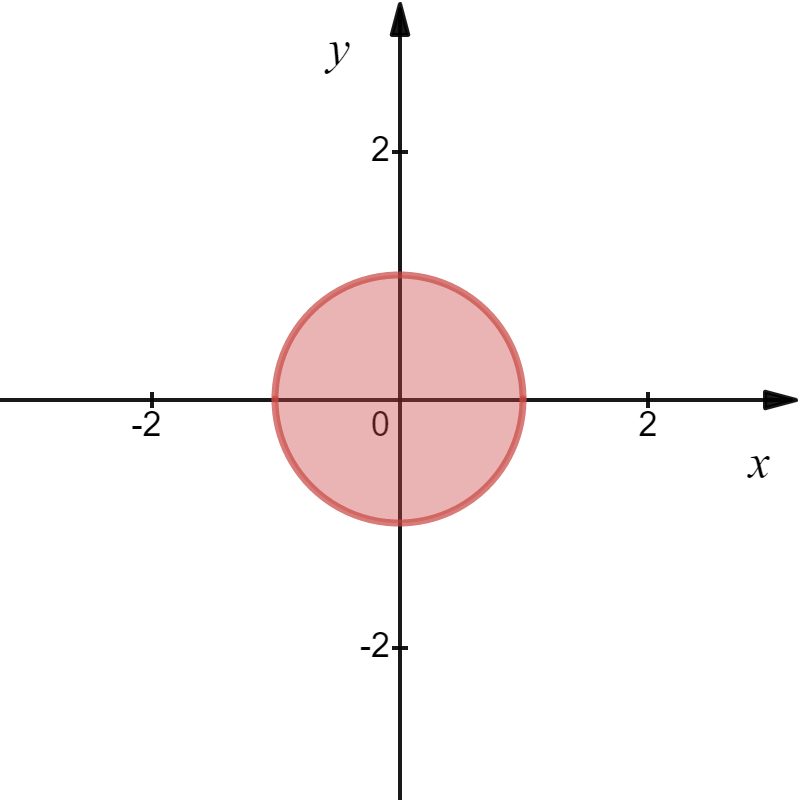
\includegraphics[width=.6\textwidth]{figures/disk.png}
    \end{figure} 
    So, if we then let $y$ range from $-1$ to $1$, we must be integrating over the unit disk in the $xy$-plane.  Then, we have $-1\leq z\leq 1$, so it must be that we are integrating over a cylindrical region.  So, to convert the whole integral to cylindrical coordinates, we note that
    \[
    dxdydz = \rho d\rho d\theta dz,
    \]
    and thus
    \[
    \int_{-1}^{1} \int_{-1}^{1} \int_{-\sqrt{1-y^2}}^{\sqrt{1-y^2}} xyz dxdydz = \int_{-1}^1 \int_{0}^{2\pi} \int_{0}^1 \rho^3 \cos(\theta)\sin(\theta)z d\rho d\theta dz.
    \]
    \item The intuition from (a) can help us since the bounds for $x$ and $y$ are similar to (a), except that we have that the radius of the circle depends is equal to $z$ and is not just fixed at 1. In other words, as $z$ increases, we are integrating over larger disks. The disks increase from a radius of 0 up to a radius of 1 linearly, so we are integrating over a solid cone!

    In fact, one way to see this is to mess with the above equations
    \begin{align*}
        -\sqrt{z^2-y^2}\leq &x \leq \sqrt{z^2-y^2} \\
        \implies ~ x^2&= z^2-y^2 \\
        \implies ~ x^2+y^2-z^2=0,
    \end{align*}
    which is the implicit equation for a double cone surface. In cylindrical coordinates, this gives us the relationship $\rho^2=z^2$ and thus $z=\pm\rho$. However, we require $0\leq z \leq 1$, so we must take $\rho=z$.  Thus, our integral then becomes
    \[
    \int_0^1 \int_{-z}^z \int_{-\sqrt{z^2-y^2}}^{\sqrt{z^2-y^2}} x^2+y^2+z^2 dx\,dy\,dz = \int_{0}^1 \int_0^{2\pi} \int_{0}^z \left(\rho^2 + z^2 \right) \rho \, d\rho \, d \theta\, dz. 
    \]
    
    \end{enumerate}
\end{solution}

\newpage
\begin{problem}
    Note that the Laplacian $\Delta$ in cylindrical coordinates is given by
    \[
        \Delta f(\rho,\theta,z) = \frac{1}{\rho} \frac{\partial}{\partial \rho} \left(\rho \frac{\partial f}{\partial \rho}\right)+\frac{1}{\rho^2}\frac{\partial^2 f}{\partial \theta^2} + \frac{\partial^2 f}{\partial z^2}.
    \]
    Compute the Laplacian of
    \[
        f(\rho,\theta,z) = \sqrt{\rho^2+z^2} z \cos(\theta).
    \]
\end{problem}
\begin{solution}
Let's compute each term and then add them together. We have
\begin{align*}
    A=\frac{1}{\rho}\frac{\partial}{\partial \rho} \left(\rho \frac{\partial f}{\partial \rho} \right) &=  \frac{z\cos \theta}{\rho} \frac{\partial}{\partial \rho} \left( \frac{\rho^2}{\sqrt{\rho^2+z^2}} \right)\\
    &=\frac{z\cos \theta}{\rho} \left(\frac{2\rho}{\sqrt{\rho^2+z^2}}-\frac{\rho}{\left(\rho^2+z^2\right)}\right)\\
    &= z\cos \theta \left( \frac{2}{\sqrt{\rho^2+z^2}} - \frac{1}{\left(\rho^2+z^2\right)}\right).
\end{align*}
Likewise, we have
\begin{align*}
    B=\frac{1}{\rho^2} \frac{\partial^2 f}{\partial \theta^2} &= -\frac{\sqrt{\rho^2+z^2}z\cos\theta}{\rho^2}.
\end{align*}  
Lastly, we have
\begin{align*}
    C=\frac{\partial^2 f}{\partial z^2} &= \cos \theta \frac{\partial}{\partial z}\frac{\partial}{\partial z} \left( z \sqrt{\rho^2+z^2}\right)\\
    &= \cos \theta \frac{\partial}{\partial z} \left( \sqrt{\rho^2+z^2}+ \frac{z^2}{\sqrt{\rho^2+z^2}}\right)\\
    &= \cos \theta \left(\frac{z}{\sqrt{\rho^2+z^2}}+\frac{2z}{\sqrt{\rho^2+z^2}}-\frac{z^3}{\left(\rho^2+z^2\right)^{3/2}}\right).
\end{align*}
Then we have that
\[
\Delta f = A+B+C.
\]
\end{solution}

\newpage
\begin{problem}
	In spherical coordinates (either implicitly or explicitly), parameterize the following objects.
	\begin{enumerate}[(a)]
		\item A solid sphere with radius 3.
		\item The surface of an infinite cone with a vertex angle of $\pi/4$.
		\item A latitudinal curve on the unit sphere at the latitude of 30$^\circ$ above the equator.
		\item A solid unit sphere with a cylinder of radius 1/2 removed from the core.
	\end{enumerate}
\end{problem}
\begin{solution} ~
 \begin{enumerate}[(a)]
    \item In this case, it's easiest to just take $0\leq r \leq 3$, $0\leq \theta < 2\pi$ and $0\leq \phi \leq \pi$.  
    \item Here, we let $\phi=\frac{\pi}{8}$ so that the vertex angle is $\frac{\pi}{4}$.  Then we let $r\in [0,\infty)$ and $\theta \in [0,2\pi)$.
    \item We can write this in spherical coordinates by noting that 30$^\circ$ is $\frac{\pi}{6}$ and that we can get $\phi(t)$ must be constant and indeed 
    \[
    \phi(t) = \frac{\pi}{2}-\frac{\pi}{6}=\frac{\pi}{3}.
    \]
    Then, since the curve is on the unit sphere, it must be that $r(t)=1$ and finally we have freedom to choose $\theta(t)$ so long as $\theta$ runs over the range $[0,2\pi)$. Most easily is to take $\theta(t)=t$ and $t\in [0,2\pi)$ to get the curve
    \[
    \curvegamma(t) = \rhat + t \thetahat +\frac{\pi}{3} \phihat.
    \]
    \item Recall that a cylinder of radius $\frac{1}{2}$ has the equation
    \[
    x^2+y^2=\frac{1}{4}.
    \]
    The unit sphere is given by $r\leq 1$ with $\theta \in [0,2\pi)$ and $\phi \in [0,\pi]$. However, one can see that for this object to be properly parameterized, we need that $r$ depends on $\phi$.  Drawing from a side profile can lead one to find that we must always have the small value for $r$ is
    \[
    r_{\textrm{min}} \sin \phi = \frac{1}{2}
    \]
    Then, it must be that at smallest $\phi = \frac{\pi}{6}$ since when $r=1$ we have $\phi = \arcsin(1/2) = \frac{\pi}{6}$.  So, the description is given by $\phi \in [\pi/6, 5\pi/6]$ with $\frac{1}{2\sin \phi} \leq r \leq 1$ and $\theta \in [0,2\pi)$.
 \end{enumerate}
\end{solution}

\newpage
\begin{problem}
    Let us see some of the benefit of using spherical coordinates. 
    \begin{enumerate}[(a)]
        \item Using the fact that 
        \[
        \rhat = \frac{x}{\sqrt{x^2+y^2+z^2}}\xhat + \frac{y}{\sqrt{x^2+y^2+z^2}}\yhat + \frac{z}{\sqrt{x^2+y^2+z^2}}\zhat,
        \]
        convert the vector field 
        \[
        \vecfieldE(x,y,z) = \begin{pmatrix} \frac{x}{(x^2+y^2+z^2)^{3/2}} \\ \frac{y}{(x^2+y^2+z^2)^{3/2}} \\ \frac{z}{(x^2+y^2+z^2)^{3/2}} \end{pmatrix},
        \] into spherical coordinates (i.e., only a function of $r$, $\theta$, $\phi$, and $\rhat$, $\thetahat$, and $\phihat$).
        \item Parameterize the surface of a sphere of radius $R$ (which we'll call $\Sigma$) as well as the outward normal vector $\unitvec$ and  in spherical coordinates.
        \item Compute the following integral using spherical coordinates that we have found:
        \[
        \iint_\Sigma \vecfieldE \cdot \unitvec d\Sigma,
        \]
        where $d\Sigma$ will be the area form in spherical coordinates.
    \end{enumerate}
\end{problem}
\begin{solution}~
\begin{enumerate}[(a)]
    \item We have
    \begin{align*}
    \vecfieldE &= \frac{x}{\left(x^2+y^2+z^2\right)^{3/2}} \xhat + \frac{y}{\left(x^2+y^2+z^2\right)^{3/2}} \yhat + \frac{z}{\left(x^2+y^2+z^2\right)^{3/2}} \zhat\\
     &= \frac{1}{x^2+y^2+z^2} \left( \frac{x}{\sqrt{x^2+y^2+z^2}} \xhat + \frac{y}{\sqrt{x^2+y^2+z^2}} \yhat + \frac{z}{\sqrt{x^2+y^2+z^2}} \zhat\right)\\
     &= \frac{1}{x^2+y^2+z^2} \rhat\\
     &= \frac{1}{r^2} \rhat.
    \end{align*}
    \item We have the parameterization of the surface of a unit sphere given by letting $r=R$ and $\theta \in [0,2\pi)$ and $\phi \in [0,\pi]$. We can use the implicit equation $f(r,\theta,\phi)=r-R$ to find the surface normal by
    \begin{align*}
        \unitvec &= \frac{\grad f}{\left| \grad f \right|} \\
        &= \frac{\grad r}{\left|\grad r\right|}\\
        &= \rhat,
    \end{align*}
    by definition. This was done in a previous homework in cartesian coordinates as well.
    \item From the previous work, we have that
    \[
    \vecfieldE \cdot \unitvec = \frac{1}{r^2}.  
    \]
    Then, this gives us
    \begin{align*}
        \iint_{\Sigma} \vecfieldE \cdot \unitvec d\Sigma &= \int_0^\pi \int_0^{2\pi} \frac{1}{R^2} R^2 \sin \phi  \, d\theta \, d\phi \\
        &= 2\pi \int_0^\pi \sin \phi \, d \phi\\
        &= 4 \pi.  
    \end{align*}
    One can notice that the radius of the sphere (so long as it is nonzero) does not come into play here.
\end{enumerate} 
\end{solution}

\newpage
\begin{problem}
    Note that the Laplacian $\Delta$ in spherical coordinates is given by
    \[
        \Delta f(r,\theta,\phi) = \frac{1}{r^2} \frac{\partial}{\partial r} \left(r^2 \frac{\partial f}{\partial r}\right)+\frac{1}{r^2 \sin^2 \phi} \frac{\partial^2 f}{\partial \theta^2} + \frac{1}{r^2 \sin\phi}\frac{\partial}{\partial \phi} \left(\sin \phi \frac{\partial f}{\partial \phi}\right).
    \]
    Compute the Laplacian of
    \[
       f(r,\theta,\phi) = r^2 \cos(\theta)\cos(\phi).
    \]
\end{problem}
\begin{solution}
 Again, we will do this piece by piece. First, we have
 \begin{align*}
    A=\frac{1}{r^2}\frac{\partial}{\partial r} \left(r^2 \frac{\partial f}{\partial r}\right)&= \frac{\cos (\theta) \cos (\phi)}{r^2}\frac{\partial}{\partial r} \left(2r^3\right) \\
    &= \frac{\cos (\theta) \cos(\phi)}{r^2} 6r^2\\
    &= 6 \cos (\theta) \cos (\phi).
 \end{align*}
 Next, we have
 \begin{align*}
    B=\frac{1}{r^2 \sin \phi} \frac{\partial^2 f}{\partial \theta^2} &= \frac{1}{r^2 \sin \phi} (-r^2\cos(\theta)\cos(\phi))\\
    &= -\frac{\cos(\theta)\cos(\phi)}{\sin\phi}
 \end{align*}
 Lastly, we have
 \begin{align*}
    C=\frac{1}{r^2\sin \phi} \frac{\partial }{\partial \phi} \left(\sin \phi \frac{\partial f}{\partial \phi}\right)&= \frac{1}{r^2\sin \phi} \frac{\partial }{\partial \phi} \left( -r^2 \cos(\theta) \sin^2(\phi)\right)\\
&=\frac{1}{r^2 \sin \phi} -2r^2 \cos(\theta)\sin(\phi)\cos(\phi)\\
&=-2\cos(\theta)\cos(\phi).
 \end{align*}
 Then,
 \[
 \Delta f = A+B+C.
 \]
\end{solution}

\end{document}